\documentclass[a4paper,oneside,reqno]{amsart}

\input{../../../../cambridge-macros.tex}

%    Set assignment information here
\newcommand{\authorname}{Feynman Liang}
\newcommand{\coursename}{MLSALT 8: Statistical Machine Translation}
\newcommand{\assignmentname}{Practical 3: Hierarchical Phrase-based Translation
with alternative grammars}

\begin{document}

\title{\coursename\\\assignmentname}

\author{\authorname}
\date{\today}

\maketitle

\section{Preliminary Questions}
\begin{enumerate}[label=\arabic*.]
  \item The language model probability is not included as a feature in the
    rulefile because it is defined for $N$-grams over the target language
    (i.e.\ English). This means that they can only be applied when:
    \begin{enumerate}
      \item A complete sequence of terminals has been derived and no
        non-terminals are remaining
      \item The identity of the previous $N-1$ terminals is known
    \end{enumerate}
    Rules containing non-terminals or yielding less than $N$ terminal symbols
    do not satisfy these requirements, hence it doesn't make sense to assign
    them a language model score.

    The language model scores could be included if:
    \begin{enumerate}
      \item The language model is a $1$-gram model, in which case the language
        model score of a rule is the joint probability of all the terminals
        derived one step after applying the rule
      \item The degenerate case where the entire sequence of non-terminals is
        derived in a single rule. The score would then be the score of the
        target sentence under the language model.
    \end{enumerate}

  \item We find that there are $20$ unique alternative translations
    \begin{lstlisting}[language=bash]
printstrings -n 10000 --input=output/example/LATS/14.fst.gz -w -u | wc -l
20
    \end{lstlisting}
    and that there are a total of 797 translation candidates (including repeated hypotheses)
    \begin{lstlisting}[language=bash]
printstrings -n 10000 --input=output/example/LATS/14.fst.gz -w | wc -l
797
    \end{lstlisting}

  \item We verify that the translation lattice has a single output translation
    \begin{lstlisting}[language=bash]
printstrings -n 10000 -u -w --input=output/example/LATS.hyp1/14.fst.gz -p | wc -l
1
    \end{lstlisting}
    and that there are a total of 83 (unique) alternative derivations generating this
    single hypothesis
    \begin{lstlisting}[language=bash]
printstrings -n 10000 -u -w --input=output/example/LATS.hyp1/14.fst.gz | wc -l
83
    \end{lstlisting}


\end{enumerate}

\section{First part}

\begin{enumerate}[label=\arabic*.]
  \item
    We translate and score the 30 sentences using grammar A:
    \begin{lstlisting}[language=bash]
hifst $DIR/configs/basic+params.features \
  --textinput=$DIR/input/test30.spa.idx \
  --rulefile=$GRAMA/r.?.gz \
  --lm=$DIR/lm/test30.news-newscomm.eng.4g/G/?.G.gz --lmn=4 \
  --range=1:30 \
  --latoutputfst=output/example/LATS.A/?.fst.gz

printstrings --r=1:30 --input=output/example/LATS.A/?.fst.gz \
  --output=outA --label-map=$SUNMAP
cat outA | sed 's/<s> //g' | sed 's/ <\/s>//g' > outA

ScoreBLEU.sh \
  -t outA \
  -r $DIR/reference/test30.eng
    \end{lstlisting}
    and peform analogous commands using grammar B.

    Translating with grammar A runs significantly faster than with
    grammar B. Grammar A attains a BLEU score of $0.4778$ while grammar B
    achieves $0.5265$.

    We post-processed the hypotheses generated by \texttt{prinstrings} (see
    usages of \texttt{sed} in code listing) because the sentence boundary
    markers ``<s>'' and ``</s>'' need to be removed for \texttt{ScoreBLEU.sh}.

  \item We first compute sentence-level BLEU scores
    \begin{lstlisting}[language=bash]
for i in {1..30}; do
  printstrings --r=$i:$i --input=output/example/LATS.A/?.fst.gz 2>/dev/null \
    | sed 's/<s> //g' | sed 's/ <\/s>//g' \
    > tmp
  scoreA=$(ScoreBLEU.sh \
    -t tmp \
    -r $DIR/reference/test30/r.$i.eng.idx \
    | cut -d ' ' -f 4)

  printstrings --r=$i:$i --input=output/example/LATS.B/?.fst.gz 2>/dev/null \
    | sed 's/<s> //g' | sed 's/ <\/s>//g' \
    > tmp
  scoreB=$(ScoreBLEU.sh \
    -t tmp \
    -r $DIR/reference/test30/r.$i.eng.idx \
    | cut -d ' ' -f 4)
  rm tmp

  print "$i,$scoreA,$scoreB"
done
    \end{lstlisting}
    and obtain the results shown in \autoref{tab:sentence-bleu}.
    \begin{table}[ht!]
      \begin{tabular}{ccc}
        \toprule
        Sentence \# & Grammar A & Grammar B \\
        \midrule
        1 & 1.0000 & 1.0000 \\
        2 & 0.2126 & 0.2163 \\
        3 & 0.1548 & 0.1579 \\
        4 & 0.0994 & 0.0994 \\
        5 & 0.3575 & 0.6865 \\
        6 & 0.2677 & 0.2677 \\
        7 & 0.2878 & 0.7277 \\
        8 & 0.6695 & 0.6695 \\
        9 & 0.4694 & 0.5405 \\
        10 & 0.8154 & 0.8154 \\
        11 & 0.2555 & 0.2623 \\
        12 & 0.2131 & 0.2131 \\
        13 & 0.8579 & 0.8606 \\
        14 & 1.0000 & 1.0000 \\
        15 & 0.4845 & 0.5428 \\
        16 & 0.6741 & 0.7268 \\
        17 & 0.2641 & 0.2641 \\
        18 & 0.2923 & 0.2923 \\
        19 & 0.8215 & 0.8215 \\
        20 & 0.7825 & 0.7825 \\
        21 & 0.5787 & 0.6901 \\
        22 & 0.8465 & 0.8465 \\
        23 & 1.0000 & 1.0000 \\
        24 & 0.8496 & 0.8496 \\
        25 & 0.2024 & 0.5933 \\
        26 & 1.0000 & 1.0000 \\
        27 & 0.2510 & 0.3493 \\
        28 & 0.0665 & 0.0665 \\
        29 & 0.0780 & 0.0768 \\
        30 & 0.3597 & 0.3475 \\
        \bottomrule
      \end{tabular}
      \caption{Sentence-level BLEU scores}
      \label{tab:sentence-bleu}
    \end{table}
    For the most part, we see that the sentence-level BLEU scores are higher
    for grammar B (e.g. sentence 5 and 7). However, not every sentence is
    translated better with B than with A (e.g. sentence 30).

    \begin{enumerate}[label=(\alph*)]
      \item
        Consider sentences 5 (\autoref{tab:s5}) and 7 (\autoref{tab:s7}).
        \begin{table}[h!]
          \begin{tabular}{p{5cm}p{10cm}}
            Input sentence & aún así sabía que nunca iba a ganar tanto como los demás . \\
            English reference & still he knew he would never earn as much as the others . \\
            Grammar A translation & even so i knew that was never going to win as much as the others . \\
            Grammar B translation & yet he knew he would never to earn as much as the others . \\
          \end{tabular}
          \caption{Sentence 5}
          \label{tab:s5}
        \end{table}
        \begin{table}[h!]
          \begin{tabular}{p{5cm}p{10cm}}
            Input sentence & el analista no considera que la volatilidad vaya a afectar a la tendencia del mercado .  \\
            English reference & the analyst does not consider that volatility is going to affect the market trend .  \\
            Grammar A translation & the analyst does not believe that the volatility will affect the tendency of the market .  \\
            Grammar B translation & the analyst does not believe that the volatility is going to affect the market trend .  \\
          \end{tabular}
          \caption{Sentence 7}
          \label{tab:s7}
        \end{table}
        Comparing the two translations, we see that grammar B's English
        hypotheses clearly improve over grammar A's. For example:
        \begin{enumerate}
          \item In sentence 5, A's translation has the incorrect verb subject
            (``\emph{i} knew'') whereas B's is correct (``\emph{he} knew'')
          \item In sentence 5, A's translation has the incorrect verb object (``knew \emph{that}'')
            whereas B's is correct (``knew \emph{he}'')
          %\item In sentence 5, A's output incorrectly uses ``was'' instead of ``would.'' As
            %a result, the conditional natue of the sentence is lost.
          \item In sentence 5, B correctly translates ``earn'' while A mistranslates to ``win''
          \item In sentence 27, grammar A's translation uses ``will'' (future facts or things
            believed certain to occur) whereas the reference
            and grammar B's translation use ``is going to'' (future predictions based
            on present evidence).
          \item In sentence 27, grammar A incorrectly outputs ``tendency of the market''
            instead of ``the market trend.''
        \end{enumerate}
        This suggests that improved sentence-level BLEU score reflects a true improvement
        in translation quality.

      \item
        Consider sentence 30 (\autoref{tab:s30}).
        \begin{table}[h!]
          \begin{tabular}{p{5cm}p{10cm}}
            Input sentence & en las filipinas se han rendido los soldados rebeldes que se habían atrincherado en un hotel en manila y habían exigido la caída de la presidente gloria macapagal arroyo .  \\
            English reference & in the phillipines , renegade soldiers surrendered after seizing a hotel in manila and demanding the overthrow of president gloria macapagal arroyo .  \\
            Grammar A translation & in the philippines have been paid soldiers rebels who had been entrenched in a hotel in manila and had demanded the fall of president gloria macapagal arroyo .  \\
            Grammar B translation & in the philippines have been paid the rebel soldiers that had been entrenched in a hotel in manila and had demanded the fall of president gloria macapagal arroyo .  \\
          \end{tabular}
          \caption{Sentence 30}
          \label{tab:s30}
        \end{table}
        In this case, the two different translations are almost identical: the only difference is
        that ``soldiers rebel who'' from grammar A's translation has been changed to
        ``the rebel soldiers that'' in grammar B's translation. Arguably, grammar B's translation
        is actually better despite a lower sentence-level BLEU.

        This example reminds us to be careful and remember that BLEU is only a
        proxy for true translation quality. Although the BLEU score has degraded,
        the translation quality is about the same for both systems.

        One explanation for this degradation in score is to note that grammar B's
        translation has one more word than grammar A's. Since BLEU is computed using
        $N$-gram precisions which favor shorter sentences (hence why a brevity penalty
        is used), the additional word in grammar B's translation could be an irrelevant
        factor which nevertheless ends up lowering BLEU.
    \end{enumerate}

  \item
    \begin{table}[h!]
      \begin{tabular}{p{5cm}p{10cm}}
        Input sentence & y después llegó la época americana .  \\
            English reference & and then the american era came .  \\
            Grammar A translation & and then came the time american .  \\
            Grammar B translation & and then came the american era .  \\
      \end{tabular}
          \caption{Sentence 27}
          \label{tab:s27}
    \end{table}

    Some main differences between rulefiles A and B for sentence 27 (\autoref{tab:s27}) include:
    \begin{enumerate}
      \item A has 104 rules B has 321
      \item A's rules only contain word and phrasal translations; hiero rules
        are absent.  This means that A cannot model arbitrarily long context
        (i.e.\ has as distortion limit) and is equivalent in expressivity to a
        phrase-based SMT system.

        In contrast, B contains hiero rules out of the $X$ non-terminal and
        hence implement hierarchical phrases, which have greater generality
        but also increased computational complexity
    \end{enumerate}

    These differences can help explain the translations produced by the two
    grammars.  The grammar A translation appears to translate the sentence
    word-for-word, translationg ``epoca'' literally to time because it failed
    to account for the context. In contrast, grammar B correctly accounts for
    the context, translating ``epoca americana'' to ``american era.''

    The reason why grammar B is able to account for context lies in the
    presence of non-terminals in its yields, ultimately allowing it to achieve
    a significantly higher BLEU score. On the other hand, it also explains why
    translating under grammar B takes more time than grammar A: the presence of
    non-terminals significantly increases the complexity of decoding because it
    leverages the full generality of Hierarchical Phrase Based Translation.

  \item
    \autoref{fig:27-a-tree} and \autoref{fig:27-b-tree} show the derivation
    trees for sentences 27 under rulesets A and B respectively.
    \begin{figure}[h!]
      \begin{center}
        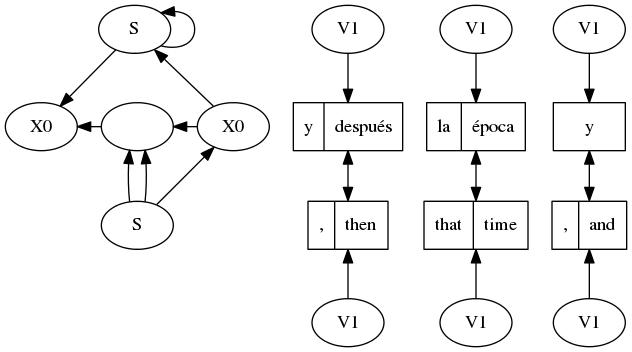
\includegraphics[scale=0.5]{../output/tree27Advn1.jpg}
      \end{center}
      \caption{Sentence 27 derivation tree under ruleset A}
      \label{fig:27-a-tree}
    \end{figure}
    \begin{figure}[h!]
      \begin{center}
        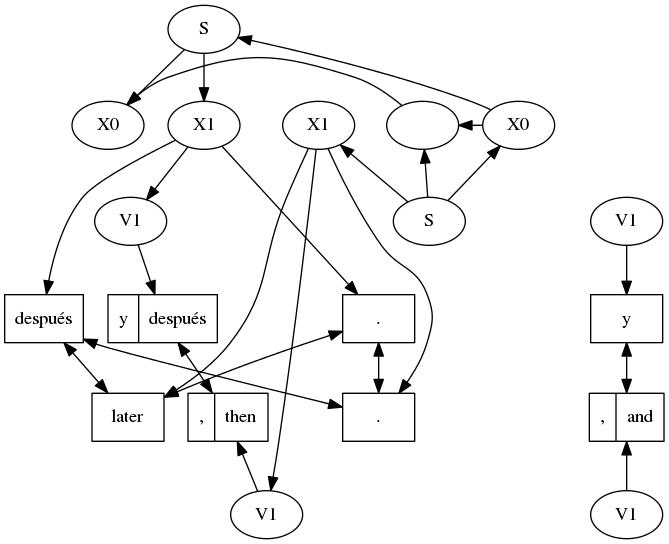
\includegraphics[scale=0.5]{../output/tree27Bdvn1.jpg}
      \end{center}
      \caption{Sentence 27 derivation tree under ruleset B}
      \label{fig:27-b-tree}
    \end{figure}
    Notice the absence of non-terminals in ruleset A's
    deivation tree (\autoref{fig:27-a-tree}), whereas ruleset B's
    tree (\autoref{fig:27-b-tree}) possesses non-terminal intermediate tree
    nodes and as a consequence exhibits much more complex structure.

    The rule sequence used for ruleset A is:
    \begin{verbatim}
X V V 0 0 0 0 0 0 0 0 0 0 0 0
S S_X S_X 0.0 0.0 0 0 -1 0 0 0 0 0 0.0 0.0
V y_después ,_then -4.0 -5.5 2 1 0 0 0 0 0 1 -6.7 -7.3
S X X 0.0 0.0 0 0 0 0 0 0 0 0 0.0 0.0
V la_época that_time -4.6 -6.0 2 1 0 0 0 0 0 1 -5.5 -8.2
V y ,_and -3.0 -1.1 2 1 0 0 0 0 0 1 -1.3 -5.0
S S_X S_X 0.0 0.0 0 0 -1 0 0 0 0 0 0.0 0.0
    \end{verbatim}
    and for ruleset B is:
    \begin{verbatim}
X V V 0 0 0 0 0 0 0 0 0 0 0 0
S S_X S_X 0.0 0.0 0 0 -1 0 0 0 0 0 0.0 0.0
V y_después ,_then -4.0 -5.5 2 1 0 0 0 0 0 1 -6.7 -7.3
X después_V1_. later_V1_. -2.5 -1.7 2 1 0 0 0 0 0 1 -6.0 -4.4
S X X 0.0 0.0 0 0 0 0 0 0 0 0 0.0 0.0
V y ,_and -3.0 -1.1 2 1 0 0 0 0 0 1 -1.3 -5.0
S S_X S_X 0.0 0.0 0 0 -1 0 0 0 0 0 0.0 0.0
    \end{verbatim}
    In particular, note the usage of the rule X $\to$ $\langle$después V1,
    later V1$\rangle$ and how it introduces non-terminal nodes into
    the derivation tree.

  \item We can align 30 sentences towards respective English references
    with grammar A using:
    \begin{lstlisting}[language=bash]
hifst $DIR/configs/basic+params.features \
  --textinput=$DIR/input/test30.spa.idx \
  --rulefile=$GRAMA/r.?.gz \
  --lm=$DIR/lm/test30.news-newscomm.eng.4g/G/?.G.gz --lmn=4 \
  --range=1:30 \
  --latoutputfst=output/example/LATS.A.towards_ref/?.fst.gz \
  --towardsreference=$DIR/reference/test30/r.?.eng.idx
    \end{lstlisting}
    and peform a similar operation with grammer B.
    Comparing the number of input sentences generating the reference for each
    grammar:

    % TODO: by examining the resulting output transducers!
    \begin{lstlisting}
integer Acnt=0
integer Bcnt=0
for i in {1..30}; do
  integer numA=$(printstrings -n 500000 -u -w --input=output/example/LATS.A.towards_ref/$i.fst.gz \
    2>/dev/null \
    | wc -l)
  integer numB=$(printstrings -n 500000 -u -w --input=output/example/LATS.B.towards_ref/$i.fst.gz \
    2>/dev/null \
    | wc -l)
  print "$i, $numA, $numB"
  Acnt+=numA
  Bcnt+=numB
done
print "Acnt: $Acnt, Bcnt: $Bcnt"
    \end{lstlisting}

    We obtain the results shown in \autoref{tab:inputs-per-ref}.
    \begin{table}[h]
      \begin{tabular}{ccc}
        \toprule
        Sentence \# & Grammar A & Grammar B \\
        \midrule
        1 & 4     & 8       \\
        2 & 1     & 1       \\
        3 & 1     & 1       \\
        4 & 1     & 1       \\
        5 & 1     & 165     \\
        6 & 1     & 1       \\
        7 & 1     & 8586    \\
        8 & 1     & 1       \\
        9 & 1     & 1       \\
        10& 48    & 122     \\
        11& 1     & 1       \\
        12& 1     & 84      \\
        13& 11070 & 51692   \\
        14& 47    & 83      \\
        15& 1     & 1       \\
        16& 1     & 1       \\
        17& 1     & 1       \\
        18& 1     & 1       \\
        19& 1     & 1       \\
        20& 52    & 166     \\
        21& 1     & 1       \\
        22& 500000& 500000  \\
        23& 2586  & 14030   \\
        24& 1     & 1       \\
        25& 1     & 282     \\
        26& 270   & 658     \\
        27& 1     & 1       \\
        28& 1     & 1       \\
        29& 1     & 1       \\
        30& 1     & 1       \\
        \hline
        Total & 514099 & 575894\\
        \bottomrule
      \end{tabular}
      \caption{Number of inputs generating the reference}
      \label{tab:inputs-per-ref}
    \end{table}
    Sentence 22 has hit the 500000 limit we used in our call to
    \texttt{printstrings}.  For all other sentences, we see that grammar B has
    many more candidate input sentences which generate the reference. This
    illustrates the additional expressivity introduced by hierarchical rules:
    derivations which were previously not possible in a phrase-based SMT system
    are now considered and hence each reference has many more derivation trees
    yielding it.

  \item No. If we compare the rule files, we see that every rule in ruleset A is
    contained in ruleset B. Hence, any derivation under A is also a valid derivation under
    B.

  \item Grammar B is strictly more expressive than grammar A. Grammar A is a simple phrase-based
    systems which translates individual phrases independently. In contrast, grammar B contains all
    the rules of grammar A plus additional heiro rules, allowing non-terminals in the derivation
    tree and hence greater expressivity (and greater computational complexity). One could
    refer to grammar A as implementing matching ``phrase-pairs'' between two languages
    and grammar B as a ``hierarchical phrase grammar'' which capitalizes on the full
    expressivity of CFGs over phrases.
\end{enumerate}

\section{Second part}

\begin{enumerate}[label=\arabic*.]
  \item

  \item
    Aligning the sentences with their English refrence with grammar C:

    \begin{lstlisting}[language=bash]
hifst $DIR/configs/basic+params.features \
  --textinput=$DIR/input/test30.spa.idx \
  --rulefile=$GRAMC/r.?.gz \
  --lm=$DIR/lm/test30.news-newscomm.eng.4g/G/?.G.gz --lmn=4 \
  --range=1:30 \
  --latoutputfst=output/example/LATS.C.towards_ref/?.fst.gz \
  --towardsreference=$DIR/reference/test30/r.?.eng.idx
    \end{lstlisting}

    Comparing the number of input sentences generating the reference
    for grammars B and C:
    \begin{lstlisting}[language=bash]
integer Bcnt=0
integer Ccnt=0
for i in {1..30}; do
  integer newB=$(printstrings -n 500000 -u -w --input=output/example/LATS.B.towards_ref/$i.fst.gz \
    2>/dev/null \
    | wc -l)
  integer newC=$(printstrings -n 500000 -u -w --input=output/example/LATS.C.towards_ref/$i.fst.gz \
    2>/dev/null \
    | wc -l)
  print "$i, $newB, $newC"
  Bcnt+=newB
  Ccnt+=newC
done
print "Bcnt: $Bcnt, Ccnt: $Ccnt"
    \end{lstlisting}

    We obtain the results % TODO
    \begin{verbatim}
    \end{verbatim}

  \item
\end{enumerate}

%\bibliographystyle{alpha}
%\nocite{*}
%\bibliography{refs}

%\appendix

%\section{Code Listings}

\end{document}
